\documentclass[submit]{../harvardml}

\course{CS1810-S26}
\assignment{Homework \#3}
\duedate{March 23, 2026 at 11:59 PM}

\usepackage{../common}
\usepackage[OT1]{fontenc}
\usepackage[colorlinks,citecolor=blue,urlcolor=blue]{hyperref}
\usepackage{graphicx}
\graphicspath{{figures/}}
\usepackage{amsmath}
\usepackage{amssymb}
\usepackage{framed}
\usepackage{color}
\usepackage{listings}
\usepackage{enumitem}
\usepackage{comment}

%%%%%%%%%%%%%%%%%%%%%%%%%%%%%%%%%%%%%%%%%%%
%% Solution environment
\usepackage{xcolor}
\newenvironment{solution}{
    \vspace{2mm}
    \color{blue}\noindent\textbf{Solution}:
}{}
%%%%%%%%%%%%%%%%%%%%%%%%%%%%%%%%%%%%%%%%%%%

\DeclareMathOperator*{\mean}{\mathbb{E}}

\lstset{
  language=Python,
  basicstyle=\ttfamily,
  keywordstyle=\color{blue}\bfseries,
  commentstyle=\color{red},
  stringstyle=\color{green},
  frame=single,
  showstringspaces=false,
}

\definecolor{verbgray}{gray}{0.9}

\lstnewenvironment{csv}{%
  \lstset{backgroundcolor=\color{verbgray},
  frame=single, % hello
  framerule=0pt,
  basicstyle=\ttfamily,
  columns=fullflexible}}{}

\begin{document}

\begin{center}
  {\Large Neural Networks and Kernels}\\
\end{center}

\subsection*{Introduction}

This homework is about neural networks and kernels.

\begin{enumerate}
  \item You'll explore how kernel functions implicitly define feature maps and how kernel ridge regression connects to predictions as weighted sums of training labels.
  \item You'll derive the backpropagation algorithm for a single-hidden-layer neural network for the binary classification task.
  \item You'll discover neural scaling laws empirically and derive optimal compute allocation strategies.
\end{enumerate}

As always, please start early and come to office hours with questions!

\subsection*{Resources and Submission Instructions}
You may want to consider the notes from Section 4 (Richer Features and Neural Networks).

Please type your solutions after the corresponding problems using this \LaTeX\ template, and start each problem on a new page.

Please submit the writeup PDF to the Gradescope assignment `HW3'. Remember to assign pages for each question.  \textbf{You must include any plots in your writeup PDF. }. Please submit your \LaTeX file and code files to the Gradescope assignment `HW3 - Supplemental.' The supplemental files will only be checked in special cases, e.g. honor code issues, etc. Your files should be named in the same way as we provide them in the repository, e.g. \texttt{hw3.pdf}, etc.

\newpage

%%%%%%%%%%%%%%%%%%%%%%%%%%%%%%%%%%%%%%%%%%%%%
% Problem 1
%%%%%%%%%%%%%%%%%%%%%%%%%%%%%%%%%%%%%%%%%%%%%

\begin{problem}[Kernels and Feature Maps, 30 pts]

In this problem, we explore how kernel functions implicitly define
feature maps and how this leads to predictions that are weighted sums of
training labels.

Recall from lecture that a kernel function $K(\boldx, \boldx')$ computes
an inner product in some feature space: $K(\boldx, \boldx') =
\bphi(\boldx)^\trans \bphi(\boldx')$, where $\bphi$ is a feature map.

\begin{enumerate}

  \item[1.] \textbf{Expanding the polynomial kernel.}
  Consider the degree-2 polynomial kernel for $\boldx \in \reals^2$:
  \[
    K(\boldx, \boldx') = (1 + \boldx^\trans \boldx')^2.
  \]

  \begin{enumerate}
    \item Writing $\boldx = (x_1, x_2)$ and $\boldx' = (x_1', x_2')$,
    expand $(1 + x_1 x_1' + x_2 x_2')^2$ and collect terms. Show that the
    result can be written as $\bphi(\boldx)^\trans \bphi(\boldx')$ for
    some feature map $\bphi : \reals^2 \to \reals^6$. State $\bphi$
    explicitly.

    \item Verify your answer with a concrete example: compute both
    $K(\boldx, \boldx')$ and $\bphi(\boldx)^\trans \bphi(\boldx')$ for
    $\boldx = (1, 0)$ and $\boldx' = (1, 1)$.
  \end{enumerate}

  \item[2.] \textbf{Visualizing the feature map.}
  We provide a synthetic dataset of concentric circles: an inner ring
  (class~0) and an outer ring (class~1). See the accompanying notebook
  for the data generation code.

  \begin{enumerate}
    \item Plot the dataset in the original space $\reals^2$.
    Are the data linearly separable? Explain briefly.

    \item Apply the feature map $\bphi$ from Part~1 to the data. Produce
    a 3D scatter plot of $(x_1,\; x_2,\; x_1^2 + x_2^2)$ with points
    colored by class. Are the data linearly separable in feature space?
    Why does this feature map help for concentric circles?

    \item Fit a ridge regression model in the feature space:
    \[
      \boldw = (\bPhi^\trans \bPhi + \lambda \ident)^{-1} \bPhi^\trans \boldy,
    \]
    where $\bPhi \in \reals^{N \times 6}$ is the feature matrix with
    $\bphi(\boldx_n)^\trans$ as its $n$th row and $\boldy \in \{0, 1\}^N$
    are the labels. Use $\lambda = 0.01$. Use pure \texttt{numpy} (no \texttt{sklearn}).
    Plot the decision boundary over the training data.
  \end{enumerate}

  \item[3.] \textbf{From feature space to kernel space.}

  In Part~2c you computed $\boldw$ and made predictions as
  $f(\boldx^*) = \bphi(\boldx^*)^\trans \boldw$, which required
  explicitly constructing the feature matrix $\bPhi$. We now show that
  the same predictions can be written as a weighted sum over training
  points, purely in terms of the kernel function $K$.

  \begin{enumerate}
    \item Let $\boldK \in \reals^{N \times N}$ be the kernel matrix
    with entries $K_{ij} = K(\boldx_i, \boldx_j)$, and define
    the weight vector
    $\balpha = (\boldK + \lambda \ident)^{-1} \boldy$.
    Show that the ridge regression prediction at a new point $\boldx^*$
    can be written as:
    \[
      f(\boldx^*) = \sum_{n=1}^{N} \alpha_n \, K(\boldx_n, \boldx^*).
    \]

    \textit{Hint}: Define $\boldw = \bPhi^\trans \balpha$ and verify
    that this $\boldw$ satisfies the ridge regression normal equations
    $(\bPhi^\trans \bPhi + \lambda \ident)\boldw = \bPhi^\trans \boldy$,
    using $\bPhi \bPhi^\trans = \boldK$.

    \item Implement kernel ridge regression using the polynomial kernel
    $K(\boldx, \boldx') = (1 + \boldx^\trans \boldx')^2$. Compute
    $\balpha = (\boldK + \lambda \ident)^{-1} \boldy$ on the
    training data. Then make a scatter plot of the training data where
    each point is sized proportionally to $|\alpha_n|$.

    \item Which points have the largest $|\alpha_n|$? Where do they tend
    to be located? Briefly explain why.

    \item In kernel ridge regression, every training point contributes to
    the prediction (all $\alpha_n \neq 0$). In a \emph{support vector
    machine} (SVM), only the training points closest to the decision
    boundary have $\alpha_n \neq 0$. These points are called
    \emph{support vectors}.

    Looking at your plot from part~(b), which training points do you
    think would be selected as support vectors? Why might it be
    useful to have most $\alpha_n = 0$?
  \end{enumerate}

  \item[4.] \textbf{The RBF kernel.}

  The radial basis function (RBF) kernel is defined as:
  \[
    K(\boldx, \boldx') = \exp\!\left(-\frac{\|\boldx - \boldx'\|^2}{2\sigma^2}\right).
  \]
  Unlike the polynomial kernel, whose degree limits it to polynomial
  decision boundaries, the RBF kernel can approximate any continuous
  decision boundary. The bandwidth $\sigma$ controls how quickly
  $K(\boldx, \boldx')$ decays with the distance between $\boldx$
  and $\boldx'$.

  \begin{enumerate}
    \item Expand $\|\boldx - \boldx'\|^2$ and use the result to write
    $K(\boldx, \boldx')$ as a product of three exponentials: one
    depending only on $\boldx$, one only on $\boldx'$ and one
    involving $\boldx^\trans \boldx'$.

    \item The other two factors depend on $\boldx$ or $\boldx'$ alone,
    so they act as scalar weights on each input. The factor involving
    $\boldx^\trans \boldx'$ is what couples the two inputs. Expand it
    as a Taylor series.

    \item The kernel trick lets us work with $K$ without ever
    computing $\bphi$ explicitly. Why is this essential for the RBF?

    \item Assume the training points are distinct. With
    $\balpha = (\boldK + \lambda \ident)^{-1} \boldy$ and
    $f(\boldx^*) = \sum_{n=1}^N \alpha_n \, K(\boldx_n, \boldx^*)$,
    show that as $\sigma \to 0$ the model classifies every training
    point correctly but predicts $f(\boldx^*) \to 0$ at any point
    not in the training set.

    \item Show that as $\sigma \to \infty$ the model predicts the
    same value at every point.
  \end{enumerate}

\end{enumerate}
\end{problem}

\newpage

\begin{solution}

\textbf{1.}

(a) Expanding $(1 + x_1 x_1' + x_2 x_2')^2$ gives us:
\begin{align*}
(1 + x_1 x_1' + x_2 x_2')^2 &= 1^2 + (x_1 x_1')^2 + (x_2 x_2')^2 + 2(1)(x_1 x_1') + 2(1)(x_2 x_2') + 2(x_1 x_1')(x_2 x_2') \\
&= 1 + 2x_1 x_1' + 2x_2 x_2' + x_1^2 (x_1')^2 + x_2^2 (x_2')^2 + 2 x_1 x_2 x_1' x_2'
\end{align*}
Now we can define the feature map $\phi : \mathbb{R}^2 \to \mathbb{R}^6$ by
\[
\phi(x) = \bigl(1,\; \sqrt{2}\,x_1,\; \sqrt{2}\,x_2,\; x_1^2,\; x_2^2,\; \sqrt{2}\,x_1 x_2\bigr)^\top
\]
This gives us:
\[
\phi(x)^\top \phi(x') = 1\cdot 1 + 2 x_1 x_1' + 2 x_2 x_2' + x_1^2 (x_1')^2 + x_2^2 (x_2')^2 + 2 x_1 x_2 x_1' x_2' = K(x, x')
\]

(b) For $x = (1, 0)$ and $x' = (1, 1)$:
\[
K(x, x') = (1 + 1\cdot 1 + 0\cdot 1)^2 = (1+1)^2 = 4
\]
$\phi(x) = (1, \sqrt{2}, 0, 1, 0, 0)^\top$ and $\phi(x') = (1, \sqrt{2}, \sqrt{2}, 1, 1, \sqrt{2})^\top$, so
\[
\phi(x)^\top \phi(x') = 1 + 2 + 0 + 1 + 0 + 0 = 4
\]

\textbf{2.}

(a) The data are not linearly separable in $\mathbb{R}^2$. The inner ring (class 0) and outer ring (class 1) are concentric circles, so any linear boundary would cut through both rings and misclassify points. We can see this in the plot:
\begin{center}
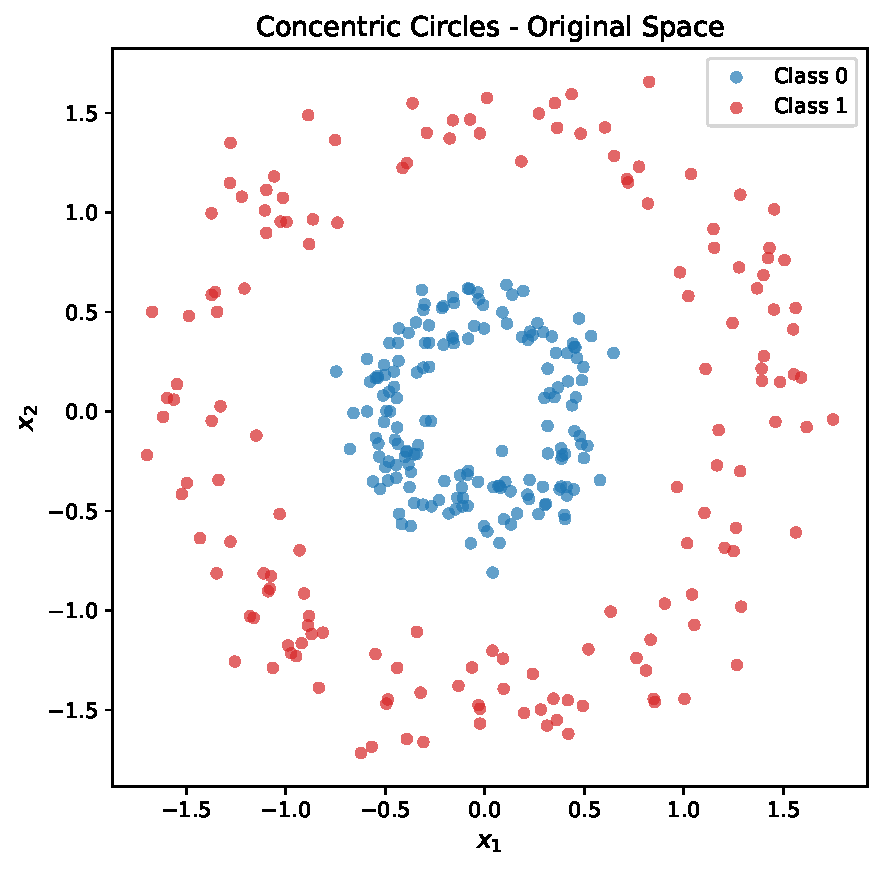
\includegraphics[width=0.5\textwidth]{p1_2a_concentric_circles.pdf}
\end{center}

(b) In feature space, the third coordinate is $x_1^2 + x_2^2 $ which is squared radius. Class 0 has smaller $r^2$ and class 1 has larger $r^2$, so a horizontal plane can separate them. The polynomial feature map helps because concentric circles differ by radius and the mapping makes radius explicit, turning a nonlinear boundary in 2D into a linear one in 3D. We can see this in the plot:
\begin{center}
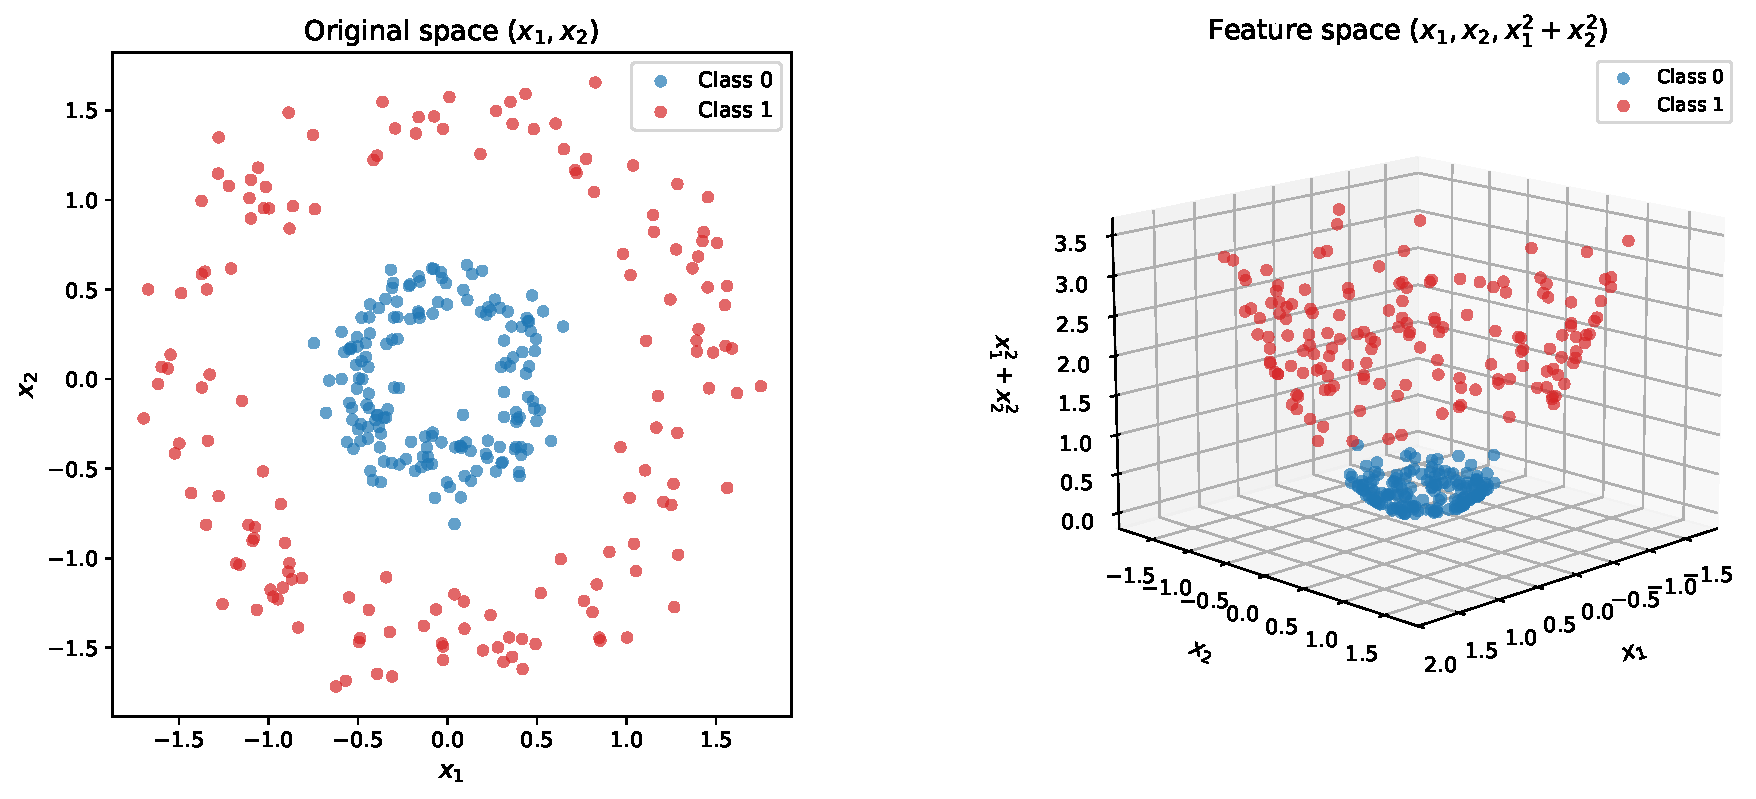
\includegraphics[width=0.8\textwidth]{p1_2b_feature_map_3d.pdf}
\end{center}

(c) The decision boundary for the specified ridge regression model is:
\begin{center}
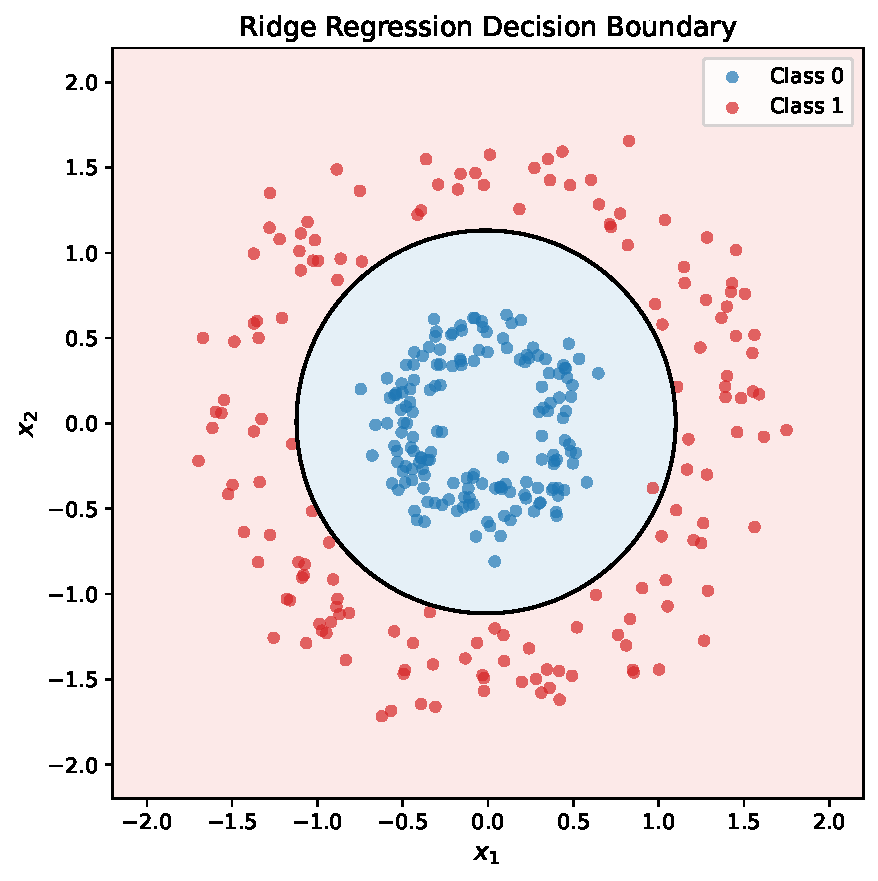
\includegraphics[width=0.5\textwidth]{p1_2c_ridge_decision_boundary.pdf}
\end{center}

\textbf{3.}

(a) We can define $w = \Phi^\top \alpha$. The ridge normal equations are $(\Phi^\top \Phi + \lambda I)w = \Phi^\top y$. By substituting $w = \Phi^\top \alpha$:
\[
(\Phi^\top \Phi + \lambda I)\Phi^\top \alpha = \Phi^\top y
\]
Left-multiply by $\Phi$g gives us $\Phi(\Phi^\top \Phi + \lambda I)\Phi^\top \alpha = \Phi \Phi^\top y$, and using $\Phi \Phi^\top = K$:
\[
(K + \lambda I) \alpha = y \Rightarrow \alpha = (K + \lambda I)^{-1} y
\]
The prediction is $f(x^*) = \phi(x^*)^\top w = \phi(x^*)^\top \Phi^\top \alpha$. The $n$th entry of $\Phi \phi(x^*)$ is $\phi(x_n)^\top \phi(x^*) = K(x_n, x^*)$, so:
\[
f(x^*) = \sum_{n=1}^{N} \alpha_n \, K(x_n, x^*)
\]

(b) The training points sized by $|\alpha_n|$:
\begin{center}
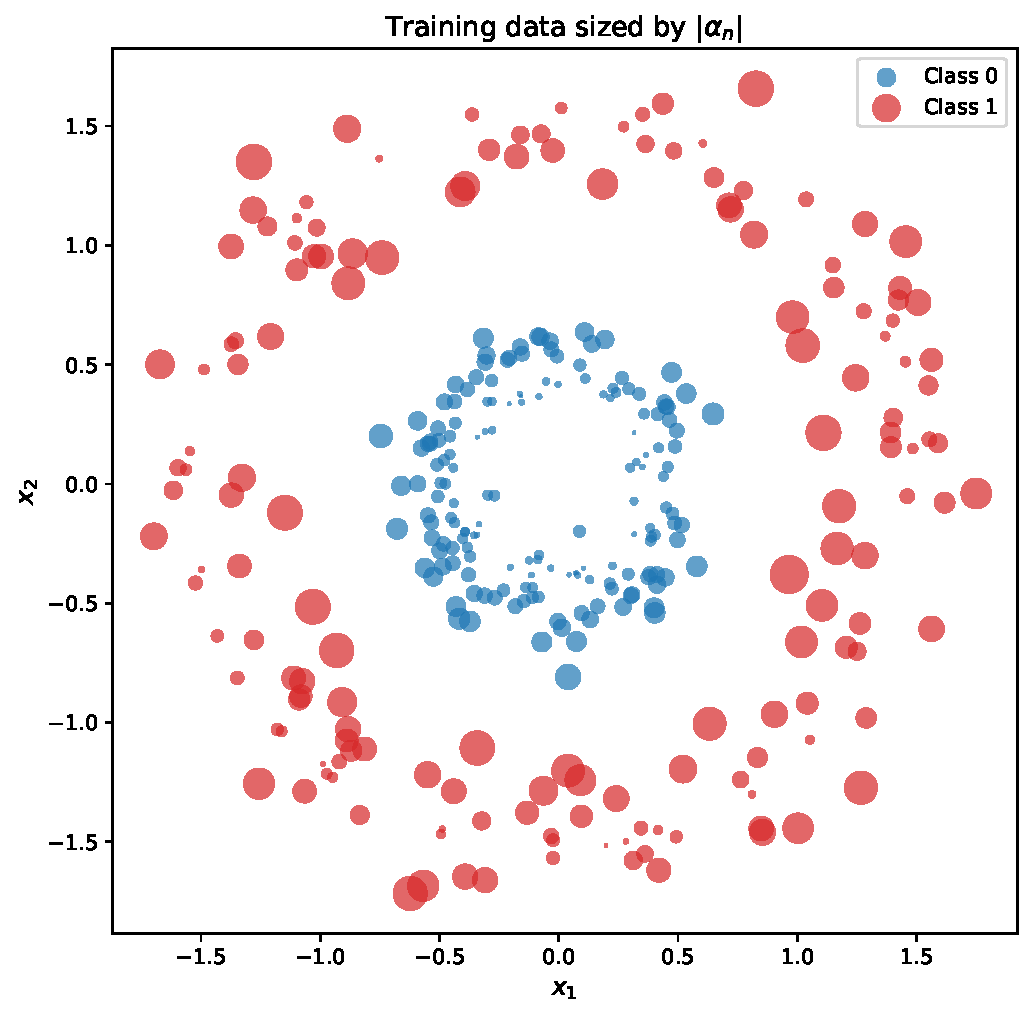
\includegraphics[width=0.5\textwidth]{p1_3b_alpha_sized.pdf}
\end{center}

(c) Points with the largest $|\alpha_n|$ tend to be near the decision boundary (the region between the inner and outer rings) or in regions where the two classes overlap. These points are most influential because they lie where the model is uncertain, small changes in their labels would most affect the fit.

(d) Support vectors would be the points near the boundary, which are the largest $|\alpha_n|$ in our plot. Having most $\alpha_n = 0$ is useful for sparsity. Predictions depend only on a few points, reducing storage and computation at test time.

\textbf{4.}

(a) We can expand $\|x - x'\|^2 = \|x\|^2 + \|x'\|^2 - 2x^\top x'$ as follows:
\[
K(x, x') = \exp\!\left(-\frac{\|x\|^2}{2\sigma^2}\right) \exp\!\left(-\frac{\|x'\|^2}{2\sigma^2}\right) \exp\!\left(\frac{x^\top x'}{\sigma^2}\right)
\]

(b) The factor $\exp(x^\top x' / \sigma^2)$ has Taylor expansion:
\[
\exp\!\left(\frac{x^\top x'}{\sigma^2}\right) = \sum_{k=0}^{\infty} \frac{1}{k!} \left(\frac{x^\top x'}{\sigma^2}\right)^k
\]

(c) The RBF kernel corresponds to an infinite dimensional feature map (the Taylor series has infinitely many terms). Computing $\phi$ explicitly is impossible. The kernel trick lets us compute $K(x, x')$ in $O(d)$ time without ever constructing $\phi$.

(d) As $\sigma \to 0$, $K(x_i, x_j) \to \delta_{ij}$ (1 if $i=j$, 0 otherwise) for distinct training points. So $K \to I$ and $\alpha \to (I + \lambda I)^{-1} y = y/(1+\lambda)$. For training point $x_n$, $f(x_n) = \sum_m \alpha_m K(x_m, x_n) \to \alpha_n \cdot 1 = y_n/(1+\lambda)$, so correct classification (threshold 0.5). For $x^* \notin \{x_1,\ldots,x_N\}$, $K(x_n, x^*) \to 0$ for all $n$, so $f(x^*) \to 0$.

(e) As $\sigma \to \infty$, $\|x - x'\|^2/(2\sigma^2) \to 0$, so $K(x, x') \to 1$ for all $x, x'$. Thus $K \to \mathbf{1}\mathbf{1}^\top$ (all ones) and $f(x^*) = \sum_n \alpha_n \cdot 1 = \mathbf{1}^\top \alpha$ is the same for every $x^*$.
\end{solution}

\newpage

%%%%%%%%%%%%%%%%%%%%%%%%%%%%%%%%%%%%%%%%%%%%%
% Problem 2
%%%%%%%%%%%%%%%%%%%%%%%%%%%%%%%%%%%%%%%%%%%%%

\begin{problem}[Neural Networks, 20 pts]

In this problem, we will take a closer look at how gradients are calculated for backpropagation with a simple multi-layer perceptron (MLP). The MLP will consist of a first fully connected layer with a sigmoid activation, followed by a one-dimensional, second fully connected layer with a sigmoid activation to get a prediction for a binary classification problem. We use non-linear activation functions as the composition of linear functions is linear. Assume bias has not been merged. Let:
\begin{itemize}
  \item $\bold{W}_1$ be the weights of the first layer, $\bold{b}_1$ be the bias of the first layer.
  \item $\bold{W}_2$ be the weights of the second layer, $\bold{b}_2$ be the bias of the second layer.
\end{itemize}

The described architecture can be written mathematically as: $$\hat{y} = \sigma(\bold{W}_2 \left[\sigma \left(\bold{W}_1 \bold{x} + \bold{b}_1\right)\right] + \bold{b}_2)$$

where $\hat{y}$ is a scalar output of the net when passing in the single datapoint $\bold{x}$ (represented as a column vector), the additions are element wise additions, and the sigmoid is an element wise sigmoid.

\begin{enumerate}
  \item Let:
        \begin{itemize}
          \item $N$ be the number of datapoints we have
          \item $M$ be the dimensionality of the data
          \item $H$ be the size of the hidden dimension of the first layer. Here, hidden dimension is used to describe the dimension of the resulting value after going through the layer. Based on the problem description, the hidden dimension of the second layer should be 1.
        \end{itemize}

        Write out the dimensionality of each of the parameters, and of the intermediate variables:

        \begin{align*}
          \bold{a}_1 & = \bold{W}_1 \bold{x} + \bold{b}_1,
                     & \bold{z}_1 = \sigma(\bold{a}_1)       \\
          a_2        & = \bold{W}_2 \bold{z}_1 + \bold{b}_2,
                     & \hat{y} = z_2 = \sigma(a_2)
        \end{align*}

        and make sure they work with the mathematical operations described above. Examining shapes is one of the key ways to debug your code, and can be done using .shape after any numpy array.

  \item  We will derive the gradients for each of the parameters, which can then be used along with gradient descent to find weights that improve our model's performance. For this question, assume there is only one datapoint $\bold{x}$, and that our loss is $L = -(y \log (\hat{y}) + (1 - y) \log (1 - \hat{y}))$. For all questions, the chain rule will be useful.
        \begin{enumerate}
          \item Find $\frac{\partial L}{\partial b_2}$.

          \item Find $\frac{\partial L}{\partial W_2^h}$, where $W_2^h$ represents the $h$th element of $\bold{W}_2$.

          \item Find $\frac{\partial L}{\partial b_1^h}$, where $b_1^h$ represents the $h$th element of $\bold{b}_1$. (\textbf{Hint}: Note that only the $h$th element of $\bold{a}_1$ and $\bold{z}_1$ depend on $b_1^h$ - this should help you with how to use the chain rule.)

          \item Find $\frac{\partial L}{\partial W_1^{h, j}}$, where  $W_1^{h,j}$ represents the element in row $h$, column $j$ in $\bold{W}_1$.

        \end{enumerate}

\end{enumerate}

\end{problem}

\newpage

\begin{framed}
  \noindent\textbf{Problem 2} (cont.)\\
  \begin{enumerate}
    \setcounter{enumi}{2}

    \item  We now explore an example of forward-mode auto-differentiation. Consider the following
          equation:

          $$
            f(x_1, x_2) = \ln (\sin (x_1)) + x_1 \exp \{ x_2 \}
          $$

          This equation can be split up using intermediate variables $v_1, \dots, v_7$ as follows:

          \begin{align*}
            v_1         & = x_1            \\
            v_2         & = \sin (v_1)     \\
            v_3         & = \ln (v_2)      \\
            v_4         & = x_2            \\
            v_5         & = \exp \{ v_4 \} \\
            v_6         & = v_1v_5         \\
            v_7         & = v_3 + v_6      \\
            f(x_1, x_2) & = v_7
          \end{align*}

          Splitting up the equation like this is very similar to what an auto-differentiation
          library would do. From these equations we can construct a \textit{computational graph}
          where each node of the graph corresponds to an input, an intermediate variable, or
          the output.

          \begin{enumerate}
            \item Let $x_1 = \frac{\pi}{6}$ and $x_2 = 1$. Calculate the values of all the
                  intermediate variables $v_1, \dots v_7$ and $f(x_1,x_2)$.
            \item Calculate the derivative of
                  all of the intermediate variables $v_1, \dots, v_7$ and
                  $f$ with respect to $x_1$ evaluated
                  at $x_1 = \frac{\pi}{6}$ and $x_2 = 1$. Remember to write out the equations before evaluating, e.g.,
                  \[
                    \frac{\partial f(x)}{\partial x} = \frac{\partial f(x)}{\partial g(x)} \frac{\partial g(x)}{\partial x}.
                  \]
          \end{enumerate}
  \end{enumerate}
\end{framed}

\newpage

\begin{solution}
\textbf{1.}

We can think of $\mathbf{x}$ as a column vector in $\mathbb{R}^M$. If we want every matrix multiply to line up, we need:
\begin{itemize}
  \item $W_1 \in \mathbb{R}^{H \times M}$, $b_1 \in \mathbb{R}^H$
  \item $a_1 = W_1 x + b_1 \in \mathbb{R}^H$, $z_1 = \sigma(a_1) \in \mathbb{R}^H$
  \item $W_2 \in \mathbb{R}^{1 \times H}$, $b_2 \in \mathbb{R}$
  \item $a_2 = W_2 z_1 + b_2 \in \mathbb{R}$, $\hat{y} = \sigma(a_2) \in \mathbb{R}$
\end{itemize}

\textbf{2.}

We use binary cross-entropy: $L = -(y \log \hat{y} + (1-y) \log(1-\hat{y}))$.

(a) If we follow the chain from $L$ to $\hat{y}$ to $a_2$, first $\frac{\partial L}{\partial \hat{y}} = -\frac{y}{\hat{y}} + \frac{1-y}{1-\hat{y}} = \frac{\hat{y} - y}{\hat{y}(1-\hat{y})}$, and next $\frac{\partial \hat{y}}{\partial a_2} = \sigma'(a_2) = \hat{y}(1-\hat{y})$. Because $a_2 = W_2 z_1 + b_2$, we have $\frac{\partial a_2}{\partial b_2} = 1$. Multiplying the pieces gives us:
\[
\frac{\partial L}{\partial b_2} = \frac{\partial L}{\partial \hat{y}} \frac{\partial \hat{y}}{\partial a_2} \frac{\partial a_2}{\partial b_2} = \frac{\hat{y} - y}{\hat{y}(1-\hat{y})} \cdot \hat{y}(1-\hat{y}) \cdot 1 = \hat{y} - y
\]

(b) If we write out $a_2 = \sum_{h'} W_2^{h'} z_1^{h'} + b_2$, the derivative with respect to one weight is simply $\frac{\partial a_2}{\partial W_2^h} = z_1^h$. Chaining as before, we get:

\[
\frac{\partial L}{\partial W_2^h} = \frac{\partial L}{\partial \hat{y}} \frac{\partial \hat{y}}{\partial a_2} \frac{\partial a_2}{\partial W_2^h} = (\hat{y} - y) \cdot z_1^h
\]

(c) Only $a_1^h$ and $z_1^h$ depend on $b_1^h$. If we walk the graph $L \to \hat{y} \to a_2 \to z_1^h \to a_1^h \to b_1^h$, we use $\frac{\partial L}{\partial a_2} = \hat{y} - y$, $\frac{\partial a_2}{\partial z_1^h} = W_2^h$, $\frac{\partial z_1^h}{\partial a_1^h} = \sigma'(a_1^h) = z_1^h(1-z_1^h)$, and $\frac{\partial a_1^h}{\partial b_1^h} = 1$. Putting it together, we get:

\[
\frac{\partial L}{\partial b_1^h} = (\hat{y} - y) \cdot W_2^h \cdot z_1^h(1-z_1^h)
\]

(d) Since $a_1^h = \sum_{j'} W_1^{h,j'} x_{j'} + b_1^h$, we get $\frac{\partial a_1^h}{\partial W_1^{h,j}} = x_j$. We can reuse the gradient from part~(c):

\[
\frac{\partial L}{\partial W_1^{h,j}} = \frac{\partial L}{\partial b_1^h} \cdot \frac{\partial a_1^h}{\partial W_1^{h,j}} = (\hat{y} - y) \cdot W_2^h \cdot z_1^h(1-z_1^h) \cdot x_j
\]

\textbf{3.}

(a) If we plug in $x_1 = \frac{\pi}{6}$ and $x_2 = 1$, we can just evaluate the graph step by step:
\begin{align*}
v_1 &= x_1 = \frac{\pi}{6}, \quad v_2 = \sin(v_1) = \frac{1}{2}, \quad v_3 = \ln(v_2) = \ln(1/2) = -\ln 2, \\
v_4 &= x_2 = 1, \quad v_5 = e^{v_4} = e, \quad v_6 = v_1 v_5 = \frac{\pi e}{6}, \quad v_7 = v_3 + v_6 = -\ln 2 + \frac{\pi e}{6}, \\
f &= v_7 = -\ln 2 + \frac{\pi e}{6} \approx -0.693 + 1.423 = 0.730
\end{align*}

(b) If we want $\partial/\partial x_1$, we propagate sensitivities forward through the same graph:
\begin{align*}
\frac{\partial v_1}{\partial x_1} &= 1, \quad \frac{\partial v_2}{\partial x_1} = \cos(v_1) \frac{\partial v_1}{\partial x_1} = \cos(\pi/6) = \frac{\sqrt{3}}{2}, \\
\frac{\partial v_3}{\partial x_1} &= \frac{1}{v_2} \frac{\partial v_2}{\partial x_1} = \frac{2 \cdot \sqrt{3}/2}{1} = \sqrt{3}, \\
\frac{\partial v_4}{\partial x_1} &= 0, \quad \frac{\partial v_5}{\partial x_1} = 0, \quad \frac{\partial v_6}{\partial x_1} = v_5 \frac{\partial v_1}{\partial x_1} + v_1 \frac{\partial v_5}{\partial x_1} = e \cdot 1 = e, \\
\frac{\partial v_7}{\partial x_1} &= \frac{\partial v_3}{\partial x_1} + \frac{\partial v_6}{\partial x_1} = \sqrt{3} + e, \quad \frac{\partial f}{\partial x_1} = \sqrt{3} + e \approx 1.732 + 2.718 = 4.450
\end{align*}
\end{solution}


\newpage

%%%%%%%%%%%%%%%%%%%%%%%%%%%%%%%%%%%%%%%%%%%%
% Problem 3
%%%%%%%%%%%%%%%%%%%%%%%%%%%%%%%%%%%%%%%%%%%%%

\begin{problem}[Neural Scaling Laws, 50 pts]
In this problem, we look pr an observation that is extremely relevant and widely utilized in industry and research.

Large-scale experiments have revealed a striking observation: the test loss of neural networks follows \textbf{power laws} in model size and dataset size. In this problem, you will discover these laws yourself on a smaller scale, use them to make predictions, and derive the optimal way to allocate a fixed compute budget.
Empirically, for many architectures and datasets, test loss $L$ follows:
\begin{equation}\label{eq:scaling}
    L(N, D) \approx \frac{a}{N^{\alpha}} + \frac{b}{D^{\beta}} + L_{\infty}
\end{equation}
where $N$ is the number of trainable parameters, $D$ is the number of training samples, and $L_\infty$ is the irreducible error (the best loss any model could achieve on this task). On a log-log plot, each term appears as a straight line.
There is no first-principles derivation of \emph{why} this particular functional form holds, it is an empirical observation. However, the form makes intuitive sense through the lens of bias-variance:
\begin{itemize}
    \item $a / N^\alpha$: \textbf{approximation error}. A small model cannot represent the true function well. As we add parameters, this error decreases --- but with diminishing returns (power law, not exponential).
    \item $b / D^\beta$: \textbf{estimation error}. Even a large model cannot learn well from too little data. More data reduces this error, again with diminishing returns.
    \item $L_\infty$: \textbf{irreducible error}. Some loss remains no matter how large the model or dataset --- due to label ambiguity, insufficient input information (e.g., low-resolution images), or inherent noise.
\end{itemize}
\subsection*{Setup: Architecture}
You will use a depth-scaled residual CNN (ResNet) with a fixed base channel width $C = 64$ and a variable number of residual blocks $K$:
\begin{center}
\begin{tabular}{@{}l@{\;}l@{}}
\textbf{Stem:} & \texttt{Conv2d}$(1, C, 3, \text{padding}=1, \text{bias}=\text{False})$ $\to$ \texttt{BatchNorm2d}$(C)$ $\to$ \texttt{ReLU} $\to$ \texttt{MaxPool2d}$(2)$ \\[6pt]
\textbf{$K \times$ ResBlock:} & each block consists of \\[2pt]
& \quad \texttt{Conv2d}$(C, C, 3, \text{padding}=1, \text{bias}=\text{False})$ $\to$ \texttt{BatchNorm2d}$(C)$ $\to$ \texttt{ReLU} \\[2pt]
& \quad $\to$ \texttt{Conv2d}$(C, C, 3, \text{padding}=1, \text{bias}=\text{False})$ $\to$ \texttt{BatchNorm2d}$(C)$ + skip $\to$ \texttt{ReLU} \\[6pt]
\textbf{Head:} & \texttt{AdaptiveAvgPool2d}$(1)$ $\to$ \texttt{Flatten} $\to$ \texttt{Linear}$(C, 10)$
\end{tabular}
\end{center}

Fashion-MNIST images are $28 \times 28$ with 1 channel. After the stem's max-pool the spatial size is $14 \times 14$; the residual blocks preserve this size; the adaptive average pool reduces it to $1 \times 1$. You are free to use \texttt{torch.nn} and \texttt{torchvision} for this problem.
\begin{enumerate}[label=(\alph*)]
%% Part (a): Discover the power laws
\item \textbf{[22 pts]} Train ResNets on Fashion-MNIST at varying scales.
\begin{enumerate}[label=(\roman*)]
    \item \textbf{[10 pts]} Write out the total parameter count $N$ as a function of $K$ (number of residual blocks) for the architecture above. Be careful: each \texttt{Conv2d} with \texttt{bias=False} has $\text{kernel}^2 \times C_{\text{in}} \times C_{\text{out}}$ parameters, each \texttt{BatchNorm2d}$(C)$ has $2C$ parameters (scale and shift), and the linear layer has $\text{in\_features} \times \text{out\_features} + \text{out\_features}$.
    Write the training code for the ResNet. The values for the different $K$ values are provided for your convenience.
    \item \textbf{[6 pts]} Fix $K = 12$ and train on random subsets of size\\ $D \in \{1000, 2000, 5000, 10000, 20000, 30000, 50000\}$. Record the final test loss for each.
    \item \textbf{[6 pts]} Make two log-log plots:
    \begin{itemize}
        \item $\log(L - \hat{L}_\infty)$ vs.\ $\log N$ (at fixed $D$)
        \item $\log(L - \hat{L}_\infty)$ vs.\ $\log D$ (at fixed $N$)
    \end{itemize}
    where $\hat{L}_\infty$ is estimated as the loss of the best configuration \emph{within each sweep} (i.e., the $K=18$ run for the model-size plot, and the $D=50000$ run for the data-size plot). This anchor point is excluded from the fit in each case.
    Fit a line to each plot. Report your estimated exponents $\hat{\alpha}$ and $\hat{\beta}$, the $R^2$ values, as well as your plots, down below.
    Discuss briefly: why do we need to subtract $\hat{L}_\infty$ before taking the log? What would the plot look like if we skipped this step? Feel free to modify the graphing code to see what it would look like, though that is not necessary.
\end{enumerate}
%% Part (b): Optimal compute allocation
\item \textbf{[10 pts]} Suppose training costs $C_{\text{compute}}$ FLOPs, and assume the approximation $C_{\text{compute}} \approx 6ND$ (forward + backward pass $\approx 6$ multiply-adds per parameter per sample).
\begin{enumerate}[label=(\roman*)]
    \item \textbf{[5 pts]} For a fixed compute budget $C_{\text{compute}}$, we want to choose $N$ and $D$ to minimize the loss in Eq.~\eqref{eq:scaling}. Using the constraint $D = C_{\text{compute}} / (6N)$, substitute into the loss and minimize over $N$. Show that the compute-optimal parameter count satisfies:
    $$
    N^*(C_{\text{compute}}) \propto C_{\text{compute}}^{\,\beta / (\alpha + \beta)}
    $$
    and the compute-optimal dataset size satisfies:
    $$
    D^*(C_{\text{compute}}) \propto C_{\text{compute}}^{\,\alpha / (\alpha + \beta)}.
    $$
    \item \textbf{[3 pts]} Plug in your empirically estimated $\hat{\alpha}$ and $\hat{\beta}$ from part (a). If you double your compute budget, by what factor should you increase $N$? By what factor should you increase $D$?
    \item \textbf{[2 pts]} The ``Chinchilla'' result (Hoffmann et al., 2022) found $\alpha \approx \beta$ for large language models, implying $N$ and $D$ should be scaled equally. If instead $\alpha \gg \beta$ (model size matters much more than data), what would the optimal strategy look like? What about $\alpha \ll \beta$?
\end{enumerate}
%% Part (c): Predict, then verify
\item \textbf{[8 pts]} This is the key test of whether scaling laws are actually useful: can you predict the performance of a model you haven't trained yet?
\begin{enumerate}[label=(\roman*)]
    \item \textbf{[4 pts]} Using \emph{only} your fitted scaling law from part (a), predict the test loss at $D = 60000$. Then actually train that model and report the true test loss.
    How close was your prediction? Discuss potential reasons for any discrepancy. \\
    Hint: What problems may arise from using $D=50000$ as your irreducible loss, and what value does it get?
    \item \textbf{[4 pts]} The $K=18$ model trained on the full dataset achieved a test cross-entropy of $0.2195$. Suppose you are limited to the $K=12$ architecture. According to your fitted data scaling law, how much training data would $K=12$ need to match $K=18$'s performance? Is this achievable? What does this tell you about the relationship between model capacity and data?
\end{enumerate}
\end{enumerate}

\end{problem}

\newpage

\begin{solution}
(a)(i) If we add up parameters block by block, it is just careful bookkeeping:

Stem: Conv2d$(1, C, 3)$: $3^2 \cdot 1 \cdot C = 9C$, BatchNorm2d$(C)$: $2C$, so the stem contributes $11C$.

Each ResBlock: Two Conv2d$(C, C, 3)$: $2 \cdot 9 \cdot C^2 = 18C^2$, Two BatchNorm2d$(C)$: $4C$, per block: $18C^2 + 4C$.

Head: Linear$(C, 10)$: $C \cdot 10 + 10 = 10C + 10$, so the head contributes $10C + 10$.

Putting it together, $N(K) = 11C + K(18C^2 + 4C) + 10C + 10 = 21C + 10 + K(18C^2 + 4C)$. If we plug in $C = 64$, we get $N(K) = 1354 + K \cdot 73984$.

(a)(ii) With $K=12$, the results are as follows:
\begin{center}
\begin{tabular}{@{}r@{\quad}r@{}}
$D$ & test CE \\ \hline
1000 & 0.71495 \\
2000 & 0.56106 \\
5000 & 0.41887 \\
10000 & 0.36048 \\
20000 & 0.29303 \\
30000 & 0.29265 \\
50000 & 0.23118 \\
\end{tabular}
\end{center}

(a)(iii) Here are the log-log plots and fits from the experiments:
\begin{center}
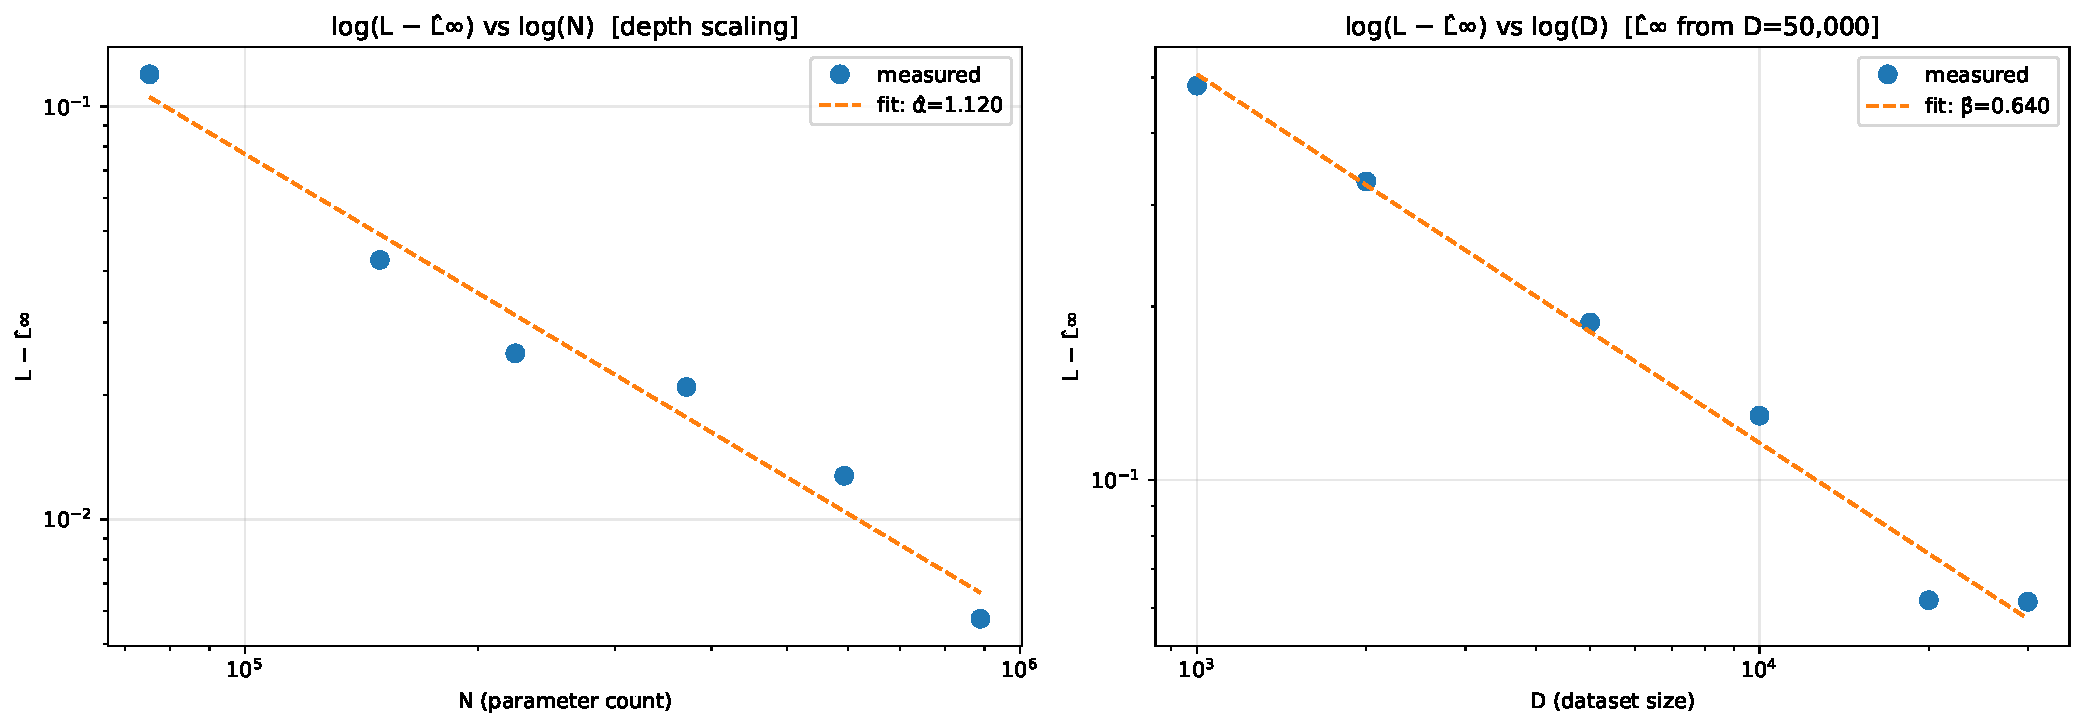
\includegraphics[width=0.9\textwidth]{p3_loglog_scaling.pdf}
\end{center}

From the linear fits on $\log(L - \hat{L}_\infty)$ (with $\hat{L}_\infty$ taken from the $K=18$ run for the model size sweep and from the $D=50000$ run for the data size sweep, and those anchors excluded from each fit), we obtain $\hat{\alpha} = 1.120$ with $R^2 = 0.968$ for the model size curve, and $\hat{\beta} = 0.640$ with $R^2 = 0.985$ for the data size curve.

We need to subtract $\hat{L}_\infty$ because if we plot $\log L$ against $\log N$ or $\log D$, the curve bends as $L$ gets close to $L_\infty$, so we do not see a clean straight line on log-log paper. If we subtract $\hat{L}_\infty$ first, then $\log(L - \hat{L}_\infty) \approx \log(a) - \alpha \log N$, which is a line with slope $-\alpha$. If we skip the subtraction, the plot tends to sag downward instead of following a power law.

(b)(i) Suppose we fix compute and use $D = C_{\text{compute}}/(6N)$. If we substitute that into Eq(1), the loss becomes a function of $N$ alone:
\[
L(N) = \frac{a}{N^\alpha} + \frac{b}{(C/(6N))^\beta} + L_\infty = \frac{a}{N^\alpha} + \frac{b \cdot 6^\beta}{C^\beta} N^\beta + L_\infty
\]
If we take a derivative with respect to $N$ and set it to zero, we get
\[
-\frac{a\alpha}{N^{\alpha+1}} + \frac{b \cdot 6^\beta}{C^\beta} \beta N^{\beta-1} = 0 \Rightarrow \frac{a\alpha}{N^{\alpha+1}} = \frac{b \cdot 6^\beta \beta}{C^\beta} N^{\beta-1}
\]
Rearranging shows how $N$ must scale with the budget:
\[
N^{\alpha+\beta} \propto C^\beta \Rightarrow N^* \propto C^{\beta/(\alpha+\beta)}, D^* = \frac{C}{6N^*} \propto C^{\alpha/(\alpha+\beta)}
\]

(b)(ii) If we double the compute budget $C_{\text{compute}}$, then $N^*$ scales by $2^{\beta/(\alpha+\beta)}$ and $D^*$ by $2^{\alpha/(\alpha+\beta)}$. Plugging in $\hat{\alpha} \approx 1.12$ and $\hat{\beta} \approx 0.64$ gives $\hat{\alpha}+\hat{\beta} \approx 1.76$, so $N^*$ should multiply by about $2^{0.64/1.76} \approx 2^{0.36} \approx 1.29$ and $D^*$ by about $2^{1.12/1.76} \approx 2^{0.64} \approx 1.55$. Here the model size exponent is larger than the data exponent, so optimal scaling allocates more compute to dataset size than to parameters when the budget doubles.

(b)(iii) If $\alpha \gg \beta$, then $\beta/(\alpha+\beta)$ is small and $\alpha/(\alpha+\beta)$ is close to $1$, so $N^*$ grows only slowly with compute while $D^*$ grows almost proportionally, the compute-optimal strategy is to scale the dataset faster than the parameter count (more FLOPs on data than on model). Intuitively, a large $\alpha$ means approximation error drops quickly as $N$ increases, while a small $\beta$ means each extra training example reduces estimation error slowly, so you need many samples. If $\alpha \ll \beta$, the exponents reverse, $N^*$ should track the budget more closely and $D^*$ grows slowly, so you prioritize larger models over more data.

(c)(i) Using only the data scaling fit from part (a), the predicted test loss at $D=60000$ (for $K=12$) is $\hat{L}(60000) = \hat{L}_\infty^{(D)} + \hat{B} \cdot 60000^{-\hat{\beta}} \approx 0.268$. Training $K=12$ on the full $D=60000$ set gave a true best test cross entropy of about $0.221$, so the prediction was off by roughly $0.047$ in absolute terms. The large gap is expected as we extrapolated beyond the largest $D$ used in the fit, and using the $D=50000$ run as $\hat{L}_\infty^{(D)}$ can overestimate the floor (that run still carries substantial finite data error). The actual run at $D=60000$ also shows that the simple two term fit misses the bend toward the true irreducible loss.

(c)(ii) To match the $K=18$ run's test loss $\approx 0.2195$, we would ask for $D$ such that $\hat{L}_\infty^{(D)} + \hat{B} D^{-\hat{\beta}} = 0.2195$ under the same data only fit. Here $\hat{L}_\infty^{(D)} \approx 0.231$ from the best $K=12$ run at $D=50000$ already exceeds $0.2195$, so the fitted equation has no positive solution for $D$. Algebraically, the model predicts that data scaling alone cannot push $K=12$ below that target. In practice, training $K=12$ on all $D=60000$ images achieved test CE $\approx 0.221$, nearly the $K=18$ number, so the fitted $\hat{L}_\infty^{(D)}$ was too pessimistic. Fashion-MNIST caps at $60{,}000$ training points anyway, so we could not test an even larger $D$. The lesson is that when approximation error dominates (small $K$), a larger model can reach a lower loss than a smaller one at the same $D$, data scaling can close much of the gap, but the pure power law fit on $D \le 50000$ does not capture the joint $(N,D)$ behavior perfectly.
\end{solution}


\newpage


%%%%%%%%%%%%%%%%%%%%%%%%%%%%%%%%%%%%%%%%%%%%%
% Name and Calibration
%%%%%%%%%%%%%%%%%%%%%%%%%%%%%%%%%%%%%%%%%%%%%

\textbf{Name}: Mert Iravul

\textbf{Collaborators and Resources}:

\end{document}
